\chapter{Kaarten beheren}\label{chapter:kaarten_beheren}

Om de opvolging van een project te kunnen garanderen moet elk teamlid kunnen aantonen welke prestaties hij geleverd heeft. Hiervoor zullen er kaarten aan het bord toegevoegd worden. Een kaart staat dan voor een taak waaraan \'e\'en of meerdere teamleden zullen werken. Op elke kaart wordt een individuele inschatting toegevoegd wanneer deze uit de ``Product backlog'' (of ``Backlog'') verplaatst wordt en nadien wordt ook elke prestatie voor deze kaart geleverd hier gelogd. Zo krijgen we nadien een overzicht of het aantal gepresteerde uren in lijn ligt met de oorspronkelijke inschatting.

\section{Kaart toevoegen}

Om een kaart aan te maken dien je volgende stappen te ondernemen:
\begin{enumerate}[nolistsep]
	\item Kies de gewenste lijst;
	\item Kies ``Een kaart toevoegen ...'';
	\item Voer de gewenste omschrijving in;
	\item Maak de kaart aan met ``Voeg toe''.
\end{enumerate}

\noindent
\\De nieuwe kaart is dan toegevoegd aan de gekozen lijst \korteverwijzing[fig:nieuwe_kaart]

\begin{figure}[h]
	\centering
	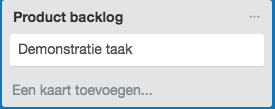
\includegraphics[scale=0.5]{./afbeeldingen/nieuwe_kaart.png}
	\caption{Voorbeeld nieuwe kaart}
	\label{fig:nieuwe_kaart}	
\end{figure} 

\section{Kaart wijzigen}

Een lege kaart zegt uiteraard niet zo veel op ons Trellobord dus deze kan op volgende manieren aangepast worden:
\begin{enumerate}[nolistsep]
	\item Naam wijzigen;
	\item Leden wijzigen;
	\item Labels beheren;
	\item Checklist beheren;
	\item Bijlage(s) beheren;
	\item Tijdsbesteding beheren \verwijzing[section:tijdsbesteding];
	\item Kaart verplaatsen, kopi\"eren of archiveren \verwijzing[chapter:kaarten_beheren].
\end{enumerate}

\noindent
\\Alle bovenstaande functionaliteiten worden toegelicht vanuit het detailscherm van een kaart \korteverwijzing[fig:detail_kaart]. Om het detailscherm van een kaart te openen volstaat het om op de kaart te ``klikken'' op het overzichtscherm van het Trellobord.

\begin{figure}[H]
	\centering
	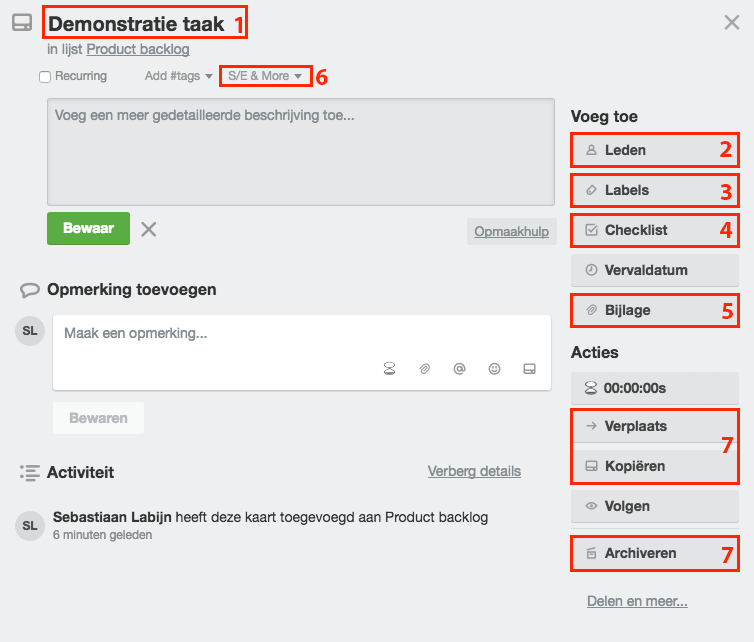
\includegraphics[scale=0.5]{./afbeeldingen/detail_kaart_genummerd.png}
	\caption{Detailscherm kaart met nummering functionaliteiten}
	\label{fig:detail_kaart}	
\end{figure} 

\paragraaf{Naam wijzigen}
\noindent
\\
Om de naam te wijzigen van een kaart kan men enerzijds in het overzichtscherm van het Trellobord op de naam klikken en deze dan aanpassen. Anderzijds kan men ook de naam aanpassen in het detailscherm op eenzelfde manier.

\paragraaf{Leden wijzigen}\label{paragraaf:leden_wijzigen}
\noindent
\\Het is soms nodig om per kaart de leden te kunnen beheren. Via deze weg kunnen we dan ook leden aan de kaart toevoegen of verwijderen zonder dat dit impact heeft op de rest van het bord. Om dit te verwezenlijken selecteer je ``leden'' en zoek dan het gewenste lid om dit toe te voegen of te verwijderen \korteverwijzing[fig:beheer_leden_kaart]

\begin{figure}[H]
	\centering
	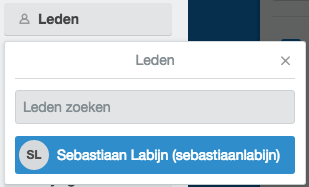
\includegraphics[scale=0.4]{./afbeeldingen/beheer_leden_kaart.png}
	\caption{Leden toevoegen/verwijderen op kaart}
	\label{fig:beheer_leden_kaart}	
\end{figure} 

\paragraaf{Labels beheren}
\noindent
\\
Om snel een overzicht te krijgen in de kaarten op een bord is het van groot belang om met labels te werken. Labels zijn kleurcodes die structuur aanbrengen in de aanwezige kaarten. Zo is het bij voorbeeld mogelijk om alle kaarten met ``geel'' te markeren die te maken hebben met een databank, alles met ``rood'' voor web, ... Op die manier kan het team snel zien welk type van kaarten er nog moeten behandeld worden of welke er allemaal afgewerkt zijn.

\noindent
\\Om een label aan kaart toe te voegen selecteer je ``labels'' en daarna kies je de gewenste kleur van het label. Het is ook mogelijk om een kleur een omschrijving te geven. Selecteer hiervoor het ``potlood'' naast de gewenste kleur. Daarnaast kan ook een nieuw label aangemaakt worden met een eigen kleur via ``Maak nieuw label aan...'' \korteverwijzing[fig:maak_label_aan]. Het gekozen label wordt dan weergegeven in het detailoverzicht van het scherm \korteverwijzing[fig:detail_kaart_labels]. Door op het labelkleur te klikken in het detailoverzicht kan je een label ook terug verwijderen van een kaart. De labels op een kaart worden ook getoond op de kaart in het Trellobord zelf \korteverwijzing[fig:bord_checklist]. Zo heb je snel een overzicht op je bord welke kaarten met welk label verbonden zijn.

\begin{figure}[H]
	\centering
	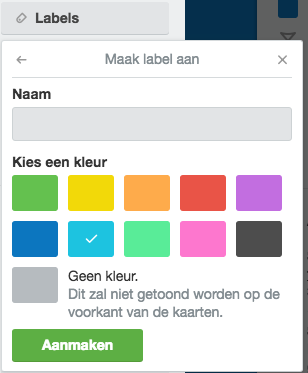
\includegraphics[scale=0.6]{./afbeeldingen/maak_label_aan.png}
	\caption{Labels aanmaken}
	\label{fig:maak_label_aan}	
\end{figure} 

\begin{figure}[H]
	\centering
	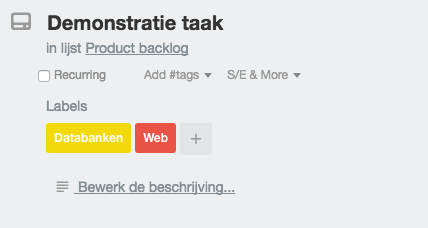
\includegraphics[scale=0.5]{./afbeeldingen/detail_kaart_labels.png}
	\caption{Kaart met labels}
	\label{fig:detail_kaart_labels}	
\end{figure} 

\paragraaf{Checklist beheren}
\noindent
\\
Checklists zijn zeer handig als een kaart uit meerdere onafhankelijke deeltaken bestaat zodat ook de voortgang binnen een kaart kan opgevolgd worden. Om een checklist toe te voegen kies je ``Checklist'' in het menu en voer dan de naam in voor de checklist. Indien er al een checklist aangemaakt was kan je hier ook keizen om items uit een vorige checklist mee te kopi\"eren. De nieuwe checklist verschijnt na bevestiging in het detailoverzicht van de kaart \korteverwijzing[fig:nieuwe_checklist].

\begin{figure}[H]
	\centering
	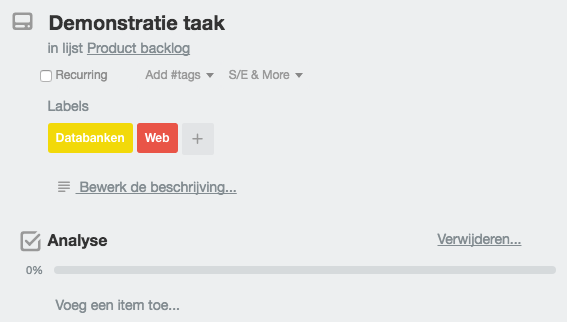
\includegraphics[scale=0.5]{./afbeeldingen/nieuwe_checklist.png}
	\caption{Kaart met lege checklist}
	\label{fig:nieuwe_checklist}	
\end{figure} 

\noindent
\\Nadien kan je in het detailzicht van de kaart ook items toevoegen aan de checklist zodat de individuele werkpunten zichtbaar worden \korteverwijzing[fig:checklist_items].

\begin{figure}[H]
	\centering
	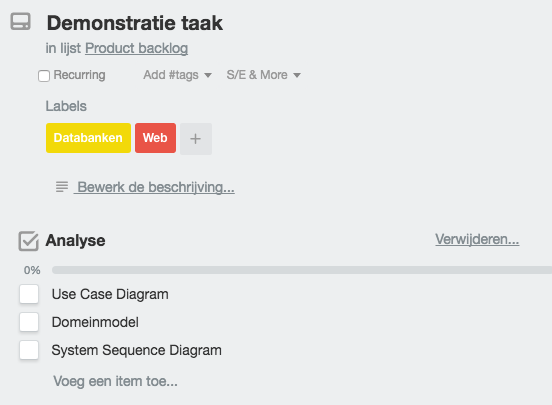
\includegraphics[scale=0.5]{./afbeeldingen/checklist_items.png}
	\caption{Checlist met items}
	\label{fig:checklist_items}	
\end{figure} 

\noindent
\\Het voordeel hiervan is dat deze voortgang ook getoond wordt op het algemene Trellobord \korteverwijzing[fig:bord_checklist]. Hierdoor hoeft het team niet telkens een kaart te openen om de voortgang te kunnen raadplegen, maar is alles snel vanuit het hoofdoverzicht te bekijken.

\begin{figure}[H]
	\centering
	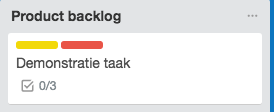
\includegraphics[scale=0.75]{./afbeeldingen/bord_checklist.png}
	\caption{Trellobord met kaart met checklist}
	\label{fig:bord_checklist}	
\end{figure} 

\paragraaf{Bijlages beheren}
\noindent
\\Bijlages kunnen een schat aan informatie zijn voor een team bij een bepaalde kaart. Deze kunnen bij voorbeeld mock-ups zijn van de layout, documenten van de opdrachtgever, gesprekken via Slack, GitHub requests... Het is dan ook heel belangrijk dat de bijlages op kaarten op een goede manier beheerd worden.
\noindent
\\\\Een nieuwe bijlage kan toegevoegd worden vanuit het detailscherm van een kaart. Hierbij kan je kiezen uit verschillende soorten bestanden:
\begin{itemize}
	\item Lokaal bestand;
	\item Trellobord of -kaart;
	\item Cloud Bestand (DropBox\footnote{\url{https://www.dropbox.com}}, Google Drive\footnote{\url{https://www.google.be/drive/about.html}}, OneDrive \footnote{\url{https://www.onedrive.com}}, ... );
	\item Hyperlink.
\end{itemize}
\noindent
De toegevoegde bijlages zijn dan ook zichtbaar in het detailzicht van de kaart \korteverwijzing[fig:bijlage_kaart]. Het is ook hier dat je bijlages kan verwijderen en eventueel extra bijlages toevoegen. Een bijlage raadplegen kan door deze aan te klikken of het bestand, indien mogelijk, te downloaden. Het is echter niet mogelijk om een bijlage aan te passen. Indien dit toch gewenst is moet de bijlage eerst verwijdert worden om ze nadien aangepast toe te voegen.

\begin{figure}[H]
	\centering
	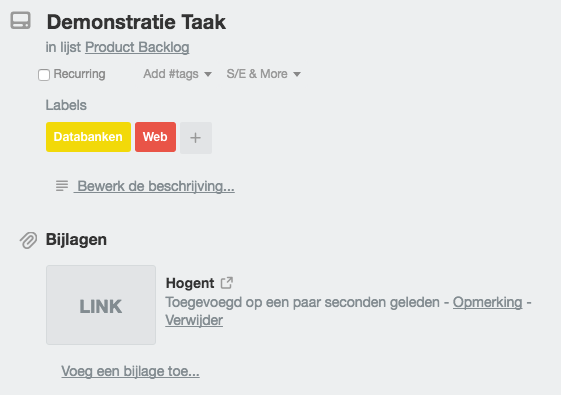
\includegraphics[scale=0.5]{./afbeeldingen/bijlage_kaart.png}
	\caption{Detailzicht van kaart met bijlage}
	\label{fig:bijlage_kaart}	
\end{figure} 

\section{Kaart(en) kopi\"eren}

Om een kaart te kopi\"eren onderneem je volgende stappen:
\begin{enumerate}[nolistsep]
	\item Open het detailzicht voor de gewenste kaart;
	\item Kies ``Kopieer'' onder ``Acties'';
	\item Kies de juiste instellingen \korteverwijzing[fig:kopieer_kaart];
	\item Bevestig met ``Kaart aanmaken''.
\end{enumerate}

\begin{figure}[H]
	\centering
	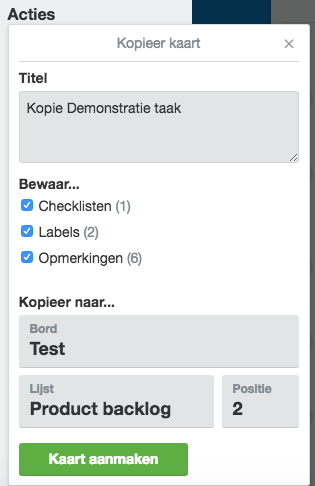
\includegraphics[scale=0.45]{./afbeeldingen/kopieer_kaart.png}
	\caption{Opties bij kopi\"eren van een kaart}
	\label{fig:kopieer_kaart}	
\end{figure} 
\noindent
\\Wil je meerdere kaarten tegelijk kop\"ieren? Herhaal dan bovenstaande stap voor elke kaart. Indien alle kaarten op een lijst moeten gekopieerd worden is het beter om de lijst zelf te kopi\"eren \verwijzing[chapter:lijsten_beheren]. 

\section{Kaart(en) verplaatsen}

Een kaart verplaatsen kan op verschillende manieren:
\begin{itemize}
	\item Wisselen van positie op eenzelfde lijst;
	\item Naar een andere lijst verplaatsen;
	\item Naar een lijst op een ander bord verplaatsen.
\end{itemize} 
\noindent
De eerste twee manieren kan je, naast de algemene methode hierna beschreven, ook verwezenlijken door de gewenste kaart vanuit het hoofdzicht van het Trellobord te verslepen naar de gewenste plaats. Wil je echter een kaart naar een ander bord verplaatsen dan kan dat enkel op de volgende manier:
\begin{enumerate}[nolistsep]
	\item Open het detailzicht voor de gewenste kaart;
	\item Kies ``Verplaatsen'' onder ``Acties'';
	\item Selecteer het gewesnte ``bord'', ``lijst'' en ``positie'' \korteverwijzing[fig:verplaats_kaart];
	\item Na bevestiging met `Verplaats'' is de kaart naar de gewenste plaats verschoven.
\end{enumerate}

\begin{figure}[h]
	\centering
	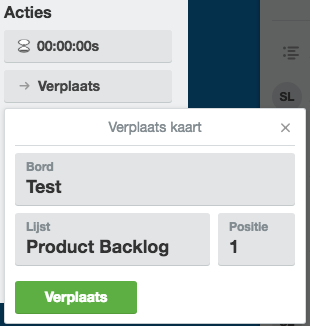
\includegraphics[scale=0.6]{./afbeeldingen/verplaats_kaart.png}
	\caption{Opties bij verplaatsen van een kaart}
	\label{fig:verplaats_kaart}	
\end{figure} 
\noindent
\\\\Om meerdere kaarten tegelijk te verplaatsen moet je bovenstaande stap voor elke te verplaatsen kaart herhalen.

\section{Kaart(en) verwijderen}

Een kaart verwijderen komt, net zoals bij lijsten, neer op het archiveren van de kaart. Om een kaart effectief van het bord te verwijderen onderneem je volgende stappen:
\begin{enumerate}[nolistsep]
	\item Open het detailzicht voor de gewenste kaart;
	\item Kies ``Archiveren'' onder ``Acties'';
	\item De kaart is nu gearchiveerd \korteverwijzing[fig:archiveer_kaart];
	\item Om de kaart definitief te verwijderen kies ``- verwijder'' OF kies ``\CircleArrowleft  Verstuur naar bord'' om archivatie ongedaan te maken;
	\item Na bevestiging is de kaart verdwenen van het bord OF teruggeplaatst op het bord.
\end{enumerate}

\begin{figure}[h]
	\centering
	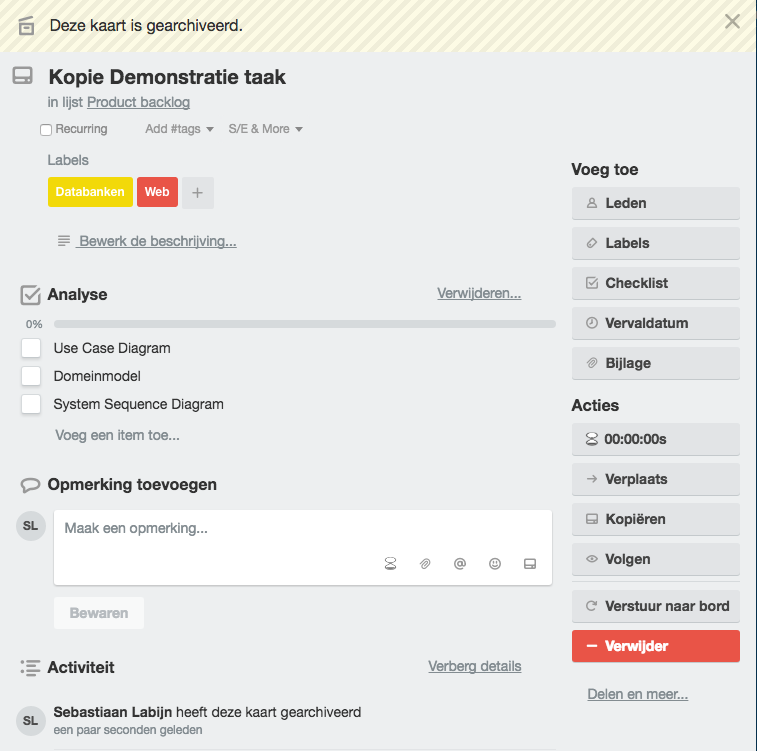
\includegraphics[scale=0.5]{./afbeeldingen/archiveer_kaart.png}
	\caption{Een gearchiveerde kaart}
	\label{fig:archiveer_kaart}	
\end{figure} 
\noindent
\\\\Om meerdere kaarten tegelijk te verwijderen moet je bovenstaande stap voor elke te verwijderen kaart herhalen.
Als je alle kaarten op een lijst wilt verwijderen is het veel effici\"enter om de lijst zelf te verwijderen \verwijzing[chapter:lijsten_beheren].

\section{Tijdsbesteding beheren}\label{section:tijdsbesteding}

Kaarten alleen op een lijst zeggen niet alles. Daarom is het van groot belang om ook de inschatting(en) en prestatie(s) te koppelen aan de juiste taken. Om dit te doen moeten de uren per teamlid toegevoegd worden op de bijhorende kaart(en). 
%De tijdsregistratie kan op twee manieren gebeuren: manueel of geautomatiseerd. \textbf{AANDACHT:} je kan enkel S uren geautomatiseerd toevoegen! Alle andere bewerkingen verlopen steeds volgens de manuele manier.

% titel in commentaar omdat geautomatiseerde methode weg(in commentaar) is
%\subsection{Manuele registratie}

\paragraaf{Toevoegen}
\\
Om de tijdseenheden toe te voegen volstaat het om volgende stappen uit te voeren:
\begin{enumerate}[nolistsep]
	\item Kies de gewenste kaart;
	\item Open het detailzicht van de kaart;
	\item Open het menu ``S/E \& more'';
	\item Kies de optie ``Add Spent' of ``Add Estimate'' afhankelijk van welke uren moeten gelogd worden;
	\item Vul de juiste waarden in voor ``S'', ``E'' en omschrijving \korteverwijzing[fig:aanmaken_prestatie];
	\item Bevestig de ingevulde uren via ``enter''.
\end{enumerate}

\begin{figure}[H]
	\centering
	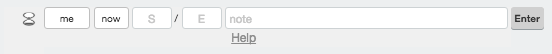
\includegraphics[scale=0.5]{./afbeeldingen/aanmaken_prestatie.png}
	\caption{Aanmaken inschatting/prestatie op een kaaart}
	\label{fig:aanmaken_prestatie}	
\end{figure} 

\noindent
\\Er werd een rij met ingevoerde uren toegevoegd \korteverwijzing[fig:aangemaakte_prestatie].
\\ \textbf{AANDACHT:} eens een rij is aangemaakt is, kan je deze NIET meer verwijderen, enkel aanpassen!

\begin{figure}[H]
	\centering
	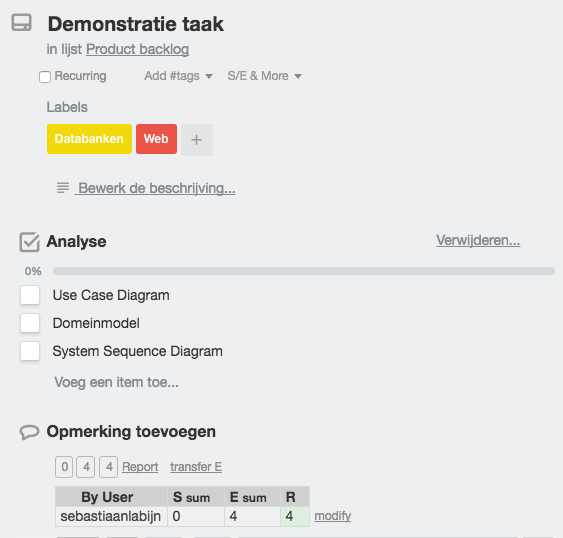
\includegraphics[scale=0.4]{./afbeeldingen/aangemaakte_prestatie.png}
	\caption{Kaart met een nieuwe inschatting}
	\label{fig:aangemaakte_prestatie}	
\end{figure} 

\paragraaf{Aanpassen}
\\
Om de tijdseenheden aan te passen volstaat het om volgende stappen uit te voeren:
\begin{enumerate}[nolistsep]
	\item Kies de gewenste kaart;
	\item Open het detailzicht van de kaart;
	\item Zoek de rij met uren die aangepast moeten worden;
	\item Selecteer ``modify'';
	\item Vul de juiste waarden in voor ``S'', ``E'' en voeg de reden van aanpassen toe indien nodig \korteverwijzing[fig:wijzigen_prestatie]
	\item Bevestig de wijziging met ``modify''
\end{enumerate}

\begin{figure}[H]
	\centering
	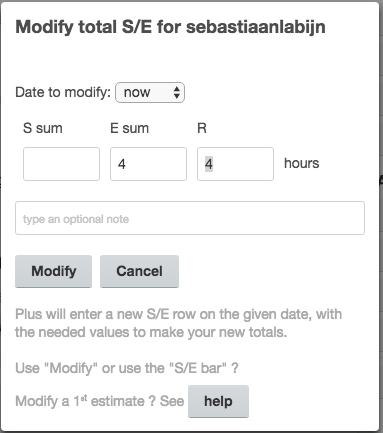
\includegraphics[scale=0.35]{./afbeeldingen/wijzigen_prestatie.png}
	\caption{Aanpassen tijdsbesteding op een kaaart}
	\label{fig:wijzigen_prestatie}	
\end{figure} 

\noindent
\\De uren op de gekozen rij werden aangepast \korteverwijzing[fig:gewijzigde_prestatie].

\begin{figure}[h]
	\centering
	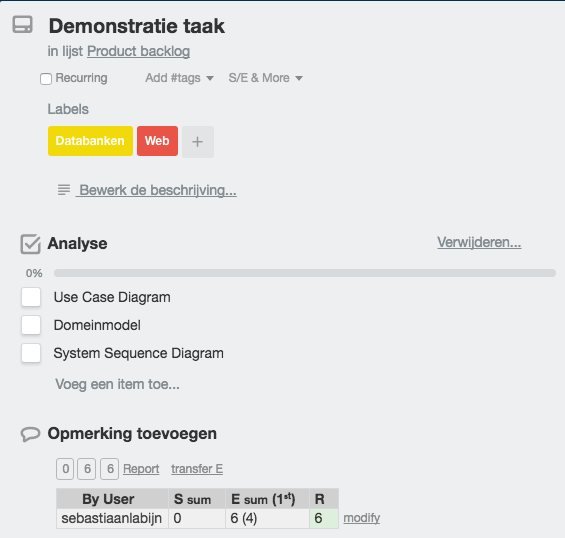
\includegraphics[scale=0.5]{./afbeeldingen/gewijzigde_prestatie.png}
	\caption{Kaart met een gewijzigde tijdsbesteding}
	\label{fig:gewijzigde_prestatie}	
\end{figure} 

\paragraaf{Uitwisselen inschatting}
\\
De techniek om uren uit te wisselen wordt vooral gebruikt indien de inschatting van de kaart niet invidueel maar op teamniveau gebeurt. De E uren worden dan toegekend aan het teamlid ``global''. Als een teamlid dan aan een kaart zal werken, transfereert hij eerst E uren van ``global'' naar zichzelf. Deze techniek kan ook gebruikt worden om tussen teamleden onderling E uren uit te wisselen. Dit doen we op een volgende manier:
\begin{enumerate}[nolistsep]
	\item Open het detailzicht van de kaart;
	\item Open het menu ``Transfer Estimate'';
	\item Voer volgende acties uit in het uitwisselscherm \korteverwijzing[fig:overzetten_prestatie]:
		\begin{enumerate}[nolistsep]
			\item ``From'': Teamlid van wie de uren overgeplaatst worden; 
			\item ``To'': Teamlid dat de uren ontvangt; 
			\item Vul het gewenste aantal E uren in;
			\item De nieuwe situatie wordt onmiddellijk in de tabel onderaan weergegeven.
		\end{enumerate}
	\item Bevestig de overplaatsing met ``enter''.
\end{enumerate}

\begin{figure}[h]
	\centering
	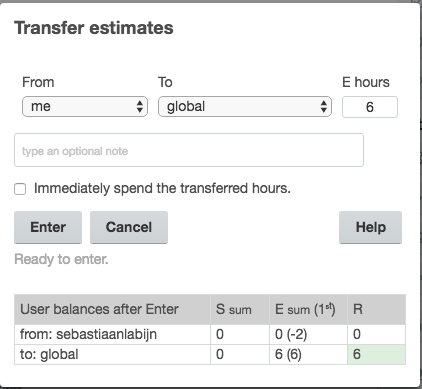
\includegraphics[scale=0.55]{./afbeeldingen/overzetten_prestatie.png}
	\caption{Overplaatsen inschatting op een kaart}
	\label{fig:overzetten_prestatie}	
\end{figure} 

\noindent
\\De uren zijn nu uitgewisseld tussen de twee teamleden \korteverwijzing[fig:overgezette_prestatie].

\begin{figure}[h]
	\centering
	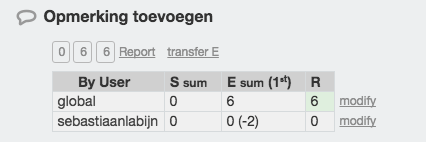
\includegraphics[scale=0.55]{./afbeeldingen/overgezette_prestatie.png}
	\caption{Kaart met een overgeplaatste prestatie}
	\label{fig:overgezette_prestatie}	
\end{figure} 

\begin{comment}
\subsection{Geautomatiseerde registratie}

Het is ook mogelijk om Trello een prestatie (ENKEL S uren) ``automatisch'' te laten registeren op een kaart. Dit gebeurt door de zandloper op de kaart, in zijn detailzicht onder acties, te activeren \korteverwijzing[fig:start_auto_reg]. 

\begin{figure}[H]
	\centering
	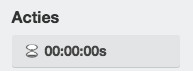
\includegraphics[scale=0.5]{./afbeeldingen/start_auto_reg.png}
	\caption{Start automatische registratie voor een prestatie}
	\label{fig:start_auto_reg}	
\end{figure} 

\noindent
\\De klok begint nu te lopen en \textbf{MOET} ook terug ``manueel'' stopgezet worden om de prestatie te be\"eindigen en nadien moet je de taak bevestigen alvorens ze effectief aan de kaart wordt toevoegd \korteverwijzing[fig:start_auto_reg]. De klok wordt dan al terug op 0 geplaatst.

\begin{figure}[H]
	\centering
	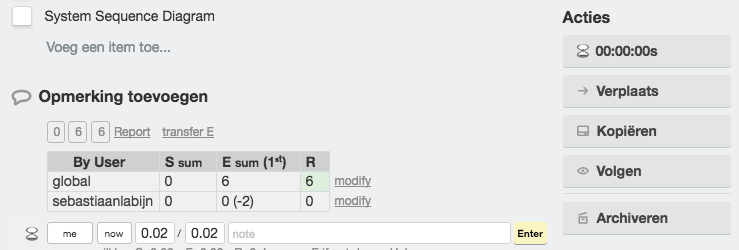
\includegraphics[scale=0.5]{./afbeeldingen/stop_auto_reg.png}
	\caption{Bevestigen automatische registratie voor een prestatie}
	\label{fig:stop_auto_reg}	
\end{figure} 
\noindent
\textbf{AANDACHT:} De browser afsluiten zal de klok NIET automatisch stopzetten! Zolang de klok loopt heb je in Chrome ook een extra venster dat je herrinnert aan de timer \korteverwijzing[fig:tijdens_auto_reg].

\begin{figure}[H]
	\centering
	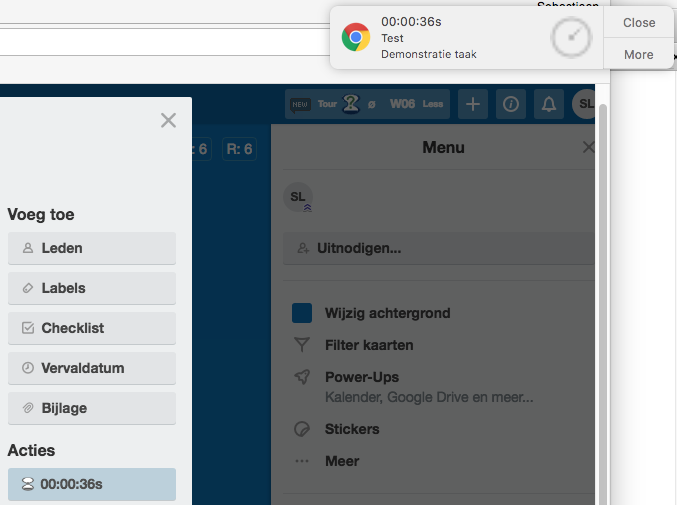
\includegraphics[scale=0.5]{./afbeeldingen/tijdens_auto_reg.png}
	\caption{Kaart tijdens automatische registratie voor een prestatie}
	\label{fig:tijdens_auto_reg}	
\end{figure} 

\noindent
\\Na bevestiging werd de prestatie aan de kaart toegevoegd \korteverwijzing[fig:prestatie_auto_reg]. Deze prestatie ziet er net uit als een manuele registratie dus er is geen onderscheid tussen beiden. Gebruik deze optie dus enkel en alleen voor kleine taken zodat je de timer zeker niet vergeet stop te zetten. Indien dit toch zo was zal je prestatie manueel moeten aanpassen, zoals reeds hiervoor beschreven.

\begin{figure}[h]
	\centering
	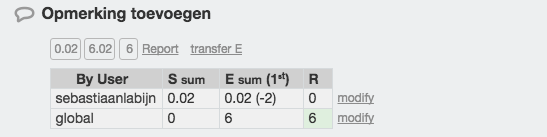
\includegraphics[scale=0.5]{./afbeeldingen/prestatie_auto_reg.png}
	\caption{Kaart met een automatische registratie voor een prestatie}
	\label{fig:prestatie_auto_reg}	
\end{figure} 
\end{comment}